% =========================================================================
% SciPost LaTeX template
% Version 1a (2016/06/14)
%
% Submissions to SciPost Journals should make use of this template.
%
% INSTRUCTIONS: simply look for the `TODO:' tokens and adapt your file.
%
% - please enable line numbers (package: lineno)
% - you should run LaTeX twice in order for the line numbers to appear
% =========================================================================


% TODO: uncommente ONE of the class declarations below
% If you are submitting a paper to SciPost Physics: uncomment next line
\documentclass{SciPost}
% If you are submitting a paper to SciPost Physics Lecture Notes: uncomment next line
%\documentclass[LectureNotes]{SciPost}
\usepackage{amsmath,amssymb,graphicx,bm,color,mathrsfs,verbatim,epstopdf,dcolumn,cancel}

%%%%%%%%%%%%%%%%%%%%%%%%%%%%%%%%%%%%%%%%%%%%%%%%%%%%%%%%%%%%%%%%

%hyperrefs
\usepackage{hyperref}
\hypersetup{ 
	colorlinks=true,
}


%define path for figs
\usepackage{graphicx}
\usepackage{caption}
\usepackage{subcaption}
% needed for \sout{}
%\usepackage[normalem]{ulem}

%%%%%%%%%%%%%%%%%%%%%%%%%%%%%%%%%%%%%%%%%%%%%%%%%%%%%%%%%%%%%%%%
%%%%%%%%%%%%%%%%%%%% Python code %%%%%%%%%%%%%%%%%%%%%%%%%%%%%%%
%%%%%%%%%%%%%%%%%%%%%%%%%%%%%%%%%%%%%%%%%%%%%%%%%%%%%%%%%%%%%%%%

\usepackage{listings}
% the following lines make sure the pdf code is copy-pastable
\usepackage{textcomp}
\usepackage[space=true]{accsupp}

\newcommand{\pdfactualhex}[3]{\newcommand{#1}{%
		\BeginAccSupp{method=hex,ActualText=#2}#3\EndAccSupp{}}}

\pdfactualhex{\pdfactualdspace}{2020}{\textperiodcentered\textperiodcentered}
\pdfactualhex{\pdfactualsquote}{27}{'}
\pdfactualhex{\pdfactualbtick}{60}{`}

% define colours 
\definecolor{deepblue}{rgb}{0,0,0.8}
\definecolor{deepred}{rgb}{1.0,0,0}
\definecolor{deepgreen}{rgb}{0,0.7,0}
\definecolor{blueviolet}{RGB}{138,43,226}
\definecolor{darkyellow}{RGB}{204,204,0}
\definecolor{codegray}{rgb}{0.6,0.6,0.6}
\definecolor{weborange}{RGB}{255,165,0}
\definecolor{gold}{RGB}{255,205,0}
\definecolor{codegreen}{rgb}{0,0.6,0}
\definecolor{codepurple}{rgb}{0.58,0,0.82}

%\definecolor{backcolour}{rgb}{0.0,0.0,0.0}
\definecolor{backcolour}{rgb}{0.95,0.95,0.92}

\lstdefinestyle{sublime}{
	backgroundcolor=\color{backcolour},   
	commentstyle=\color{deepgreen},
	keywordstyle=\color{deepred},
	numberstyle=\tiny,
	stringstyle=\color{weborange},
	basicstyle=\small\ttfamily, %\footnotesize,
	breakatwhitespace=false,         
	breaklines=true,                 
	captionpos=t,                    
	keepspaces=true,                 
	numbers=left,                    
	numbersep=5pt,                  
	showspaces=false,                
	showstringspaces=false,
	showtabs=false,                  
	tabsize=4,
	columns=flexible,
	emptylines=10000,
	literate={'}{\pdfactualsquote}1{`}{\pdfactualbtick}1{\ \ }{\pdfactualdspace}2,
	inputpath=./anc,
%	inputpath=anc/,
	keywords={lambda,xrange,abs,for,return},
}
\lstset{style=sublime,language=Python}

% change default listings caption title
\renewcommand{\lstlistingname}{QuSpin \emph{Example Code}}% Listing -> q\spin\ Example Code


%%%%%% the following lines put the slashed zero in the code environtmnet listings

\usepackage{marvosym,etoolbox}
% this replaces 0 with \0 in lstings
\lstset{literate={0}{\0}1{0\ }{\0\ }2}

\renewcommand*\ttdefault{txtt}
\usepackage[T1]{fontenc}
\usepackage{graphicx}
% defines \0 as mirro of 0
\newcommand\0{\scalebox{-1}[1]{0}}
% fix for \texttt and \ttfamily
\let\svttfamily\ttfamily
\let\svtexttt\texttt
\catcode`0=\active
\def0{\0}
\renewcommand\ttfamily{\svttfamily\catcode`0=\active }
\renewcommand\texttt{\bgroup\ttfamily\texttthelp}
\def\texttthelp#1{#1\egroup}
\catcode`0=12 %

%%%%%%%


%%%%%%%%%%%%%%%%%%%%%%%%%%%%%%%%%%%%%%%%%%%%%%%%%%%%%%%%%%%%%%%%
%%%%%%%%%%%%%%%%%%%%% qspin logo %%%%%%%%%%%%%%%%%%%%%%%%%%%%%%%
%%%%%%%%%%%%%%%%%%%%%%%%%%%%%%%%%%%%%%%%%%%%%%%%%%%%%%%%%%%%%%%% 

%\usepackage{upgreek}
%\newcommand{\qspin}{$\mathcal{Q}^{\mathrm{u}}\!\mathcal{S}\uprho\mathrm{\text{\textexclamdown}}\mathcal{N}$}


%%%%%%%%%%%%%%%%%%%%%%%%%%%%%%%%%%%%%%%%%%%%%%%%%%%%%%%%%%%%%%%%
%%%%%%%%%%%%  vertical text on the right %%%%%%%%%%%%%%%%%%%%%%%
%%%%%%%%%%%%%%%%%%%%%%%%%%%%%%%%%%%%%%%%%%%%%%%%%%%%%%%%%%%%%%%%
\usepackage{background}
\usepackage{geometry}

\definecolor{textcolor}{HTML}{0A75A8}
\newcommand\Text{ \emph{to report a bug pls visit https://github.com/weinbe58/QuSpin/issues} }

\SetBgColor{textcolor}
\SetBgOpacity{0.5}
\SetBgAngle{-90}
\SetBgPosition{current page.center}
\SetBgVshift{0.35\textwidth}
\SetBgScale{1.8}
\SetBgContents{\sffamily\Text}
%%%%%%%%%%%%%%%%%%%%%%%%%%%%%%%%%%%%%%%%%%%%%%%%%%%%%%%%%%%%%%%% 

%\usepackage{ulem}

\newcommand*{\red}{\textcolor{red}}
\newcommand*{\blue}{\textcolor{blue}}
\newcommand*{\cyan}{\textcolor{cyan}}
\newcommand*{\green}{\textcolor{green}}



\begin{document}
% TODO: write your article's title here. 
% The article title is centered, Large boldface, and should fit in two lines
\begin{center}{\Large \textbf{
QuSpin: a Python Package for Dynamics and Exact Diagonalisation of Quantum Many Body Systems.\\
\large Part II: bosons, fermions and higher spins
}}\end{center}

% TODO: write the author list here. Use initials + surname format.
% Separate subsequent authors by a comma, omit comma at the end of the list.
% Mark the corresponding author with a superscript *. 
\begin{center}
Phillip Weinberg\textsuperscript{*} and Marin Bukov
\end{center}

% TODO: write all affiliations here. 
% Format: institute, city, country
\begin{center}
Department of Physics, Boston University, \\
590 Commonwealth Ave., Boston, MA 02215, USA
\\
% TODO: provide email address of corresponding author
* weinbe58@bu.edu
\end{center}

\begin{center}
\today
\end{center}

% For convenience during refereeing: line numbers
%\linenumbers

\section*{Abstract}
{\bf 
We present a major update to QuSpin, \emph{SciPostPhys.2.1.003}, -- an open-source Python package for exact diagonalization and quantum dynamics of boson, fermion and spin many-body systems, supporting the use of various symmetries in 1-dimension and (imaginary) time evolution. We explain how to use the new features of QuSpin using six detailed examples of various complexity: (i)... This easily accessible package can serve various purposes, including educational and cutting-edge experimental and theoretical research.
}


% TODO: include a table of contents (optional)
% Guideline: if your paper is longer that 6 pages, include a TOC
% To remove the TOC, simply cut the following block
\vspace{10pt}
\noindent\rule{\textwidth}{1pt}
\tableofcontents\thispagestyle{fancy}
\noindent\rule{\textwidth}{1pt}
\vspace{10pt}


\section{What can QuSpin be Useful for?}
\label{sec:intro}

Understanding the physics of many-body quantum condensed matter systems often involves a great deal of numerical simulations, be it to gain intuition about the complicated problem of interest, or because the latter does not admit an analytical solution which can be expressed in a closed form. This motivated the development of open-source packages [CITE], the purpose of which is to facilitate the study of condensed matter systems without the need to understand and implement complicated numerical methods which required years to develop. Here, we report a major upgrade to QuSpin~\cite{weinberg_17_quspin} -- a Python library for exact diagonalisation (ED) and simulation of the dynamics of quantum many-body systems. 

Although ED methods are vastly outperformed by more sophisticated numerical techniques in the study of equilibrium systems~[CITE], as of present date ED remains essential for most dynamical non-equilibrium problems. The reason for this often times relies on the fact that the underlying physics of these problems cannot be explained without taking into consideration the contribution from high-energy states excited during the evolution. Some prominent examples of such problems include the study of many-body localisation (MBL) [CITE], the Eigenstate Thermalisation hypothesis [CITE], quantum quench dynamics [CITE], periodically-driven systems [CITE], adiabatic and counter-diabatic state preparation, applications of Machine Learning to non-equilibrium physics [CITE], and many more \cyan{\bf did I forget smth important?}.

It is, thus, arguably useful to have a toolbox available which allows one to quickly simulate and study these and related nonequilibrium problems. As such, QuSpin offers easy access to performing numerical simulations, which can facilitate the development and inspiration of new ideas and the discovery of novel phenomena, eliminating the cost of spending time to develop a reliable code. Besides theorists, the new version of QuSpin will hopefully even prove valuable to experimentalists working on problems containing dynamical setups, as it can help students and researchers focus on making the experiment run, rather than worrying about writing the supporting simulation code. Last but not least, with the computational processing power growing higher than ever before, the role played by simulations for theoretical research becomes increasingly more important too. It can, therefore, be expected that in the near future quantum simulations become an integral part of the standard physics university curriculum, and having easily accessible toolboxes, such as QuSpin, is one of the required prerequisites.


\section{How do I use the New Features of QuSpin?}
\label{sec:examples}

New in QuSpin 2.0, we have added the following features and toolboxes:
\begin{itemize}
	\item ...
\end{itemize}

\emph{Installing QuSpin is quick and efficient; just follow the steps outlined in App.~\ref{app:install}.}\\

\noindent Before we carry one, we refer the interested reader to examples (i)-(iv) from the original QuSpin paper~\cite{weinberg_17_quspin}. The examples below focus predominantly on the newly introduced features, and are thus to be considered complementary. We emphasize that, since they serve the purpose of explaining how to use QuSpin, for the sake of brevity we shall not discuss the interesting physics related to the interpretation of the results.

\subsection{The Spectrum of the Transverse Field Ising Model and the Jordan-Wigner Transformation}
\label{subsec:JW}

This example shows how to
\begin{itemize}
	\item construct fermionic hopping, $p$-wave pairing and on-site potential terms, and spin$-1/2$ interactions and transverse fields,
	\item implement periodic and anti-periodic boundary conditions with translation and parity (reflection) symmetries,
	\item use particle conservation modulo $2$, spin inversion, reflection, and translation symmetries,
	\item handle the default built-in particle conservation and symmetry checks,
	\item obtain the spectrum of a QuSpin Hamiltonian.
\end{itemize}

\noindent\emph{Physics Setup---}The transverse field Ising (TFI) chain is paradigmatic in our understanding of quantum phase transitions, since it represents an exactly solvable model[CITE Sachdev]. The Hamiltonian is given my
\begin{equation}
H=\sum_{j=0}^{L-1}-J\sigma^z_{j+1}\sigma^z_j - h\sigma^x_j,
\label{eq:TFIM}
\end{equation} 
where the nearest-neighbour (nn) spin interaction is $J$, $h$ denotes the transverse field, and $\sigma^\alpha_j$ are the Pauli spin-$1/2$ matrices. We use periodic boundary conditions and label the $L$ lattice sites $0,\dots,L-1$ to conform with Python's convention. This model has gapped, fermionic elementary excitations, and exhibits a phase transition from an antiferromagnet to a paramagnet at $\left(h/J\right)_c=1$ \cyan{CHECK!}. This Hamiltonian possesses the symmetries: magnetisation conservation, parity (reflection about the centre of the chain), spin inversion, and (many-body) momentum conservation.

In one dimension, the TFI Hamiltonian can be mapped to spinless $p$-wave superconducting fermions via the Jordan-Wigner (JW) transformation[CITE Sachdev, other paper]:
\begin{equation}
c_i=\prod_{j<i}\sigma^z_j\sigma^-_i,\qquad c^\dagger_i=\prod_{j<i}\sigma^z_j\sigma^+_i,
\label{eq:JW_transf}
\end{equation} 
where the fermionic operators satisfy $\{c_i,c^\dagger_j\}=\delta_{ij}$. The Hamiltonian is readily shown to take the form
\begin{equation}
H=\sum_{j=0}^{L-1}J\left(-c^\dagger_jc_{j+1} + c_jc^\dagger_{j+1} \right) +J\left( -c^\dagger_jc^\dagger_{j+1} + c_jc_{j+1}\right) + 2h\left(n_j-\frac{1}{2}\right).
\label{eq:TFIM_fermion}
\end{equation}
In the fermionic representation, the spin $zz$-interaction maps to nn hopping and a $p$-wave pairing term with coupling constant $J$, while the transverse field translates to an on-site potential shift of magnitude $h$. In view of the QuSpin implementation of the model, we have ordered the terms such that the site index is growing to the right which comes at the cost of a few negative signs due to the fermion statistics. The fermion Hamiltonian posses the symmetries: particle conservation modulo $2$, parity and (many-body) ``momentum'' conservation.

Here, we are interested in studying the spectrum of the TFI model in both the spin and fermion representation. However, if one naively carries out the JW transformation, and computes the spectra of Eqs.~\eqref{eq:TFIM} and~\eqref{eq:TFIM_fermion}, one might be surprised that they do not match exactly. The reason lies in the form boundary condition required to make the JW mapping exact -- a subtle issue often left aside in favour of discussing the interesting physics of the TFI model. 

Recall that the starting point is the periodic boundary condition imposed on the spin Hamiltonian~\ref{eq:TFIM}. Due to the symmetries of the spin Hamiltonian~\eqref{eq:TFIM}, we can define the JW transformation on every symmetry sector separately. To make the JW mapping exact, we supplement Eq.~\eqref{eq:JW_transf} with the following boundary conditions: (i) the negative spin-inversion symmetry sector maps to the fermion Hamiltonian~\eqref{eq:TFIM_fermion} with \emph{periodic} boundary conditions (PBC); (ii) the positive spin-inversion symmetry sector maps to the fermion Hamiltonian~\eqref{eq:TFIM_fermion} with \emph{anti-periodic} boundary conditions (APBC). Anti-periodic boundary conditions differ from PBC by a negative sign attached to all coupling constants that cross a single, fixed lattice bond (the bond itself is arbitrary as all bonds are equal for PBC). APBC and PBC are special cases of the more general, twisted boundary conditions, where instead of a negative sign, one attaches a phase factor.

In the following, we show how to compute the spectra of the Hamiltonians in Eqs.~\eqref{eq:TFIM} and~\eqref{eq:TFIM_fermion} with the correct boundary conditions. Figure~\ref{fig:JW} shows that they match exactly in both the PBC and APBC cases.

\begin{figure}[t!]
	\centering
	\begin{subfigure}[b]{0.496\textwidth}
		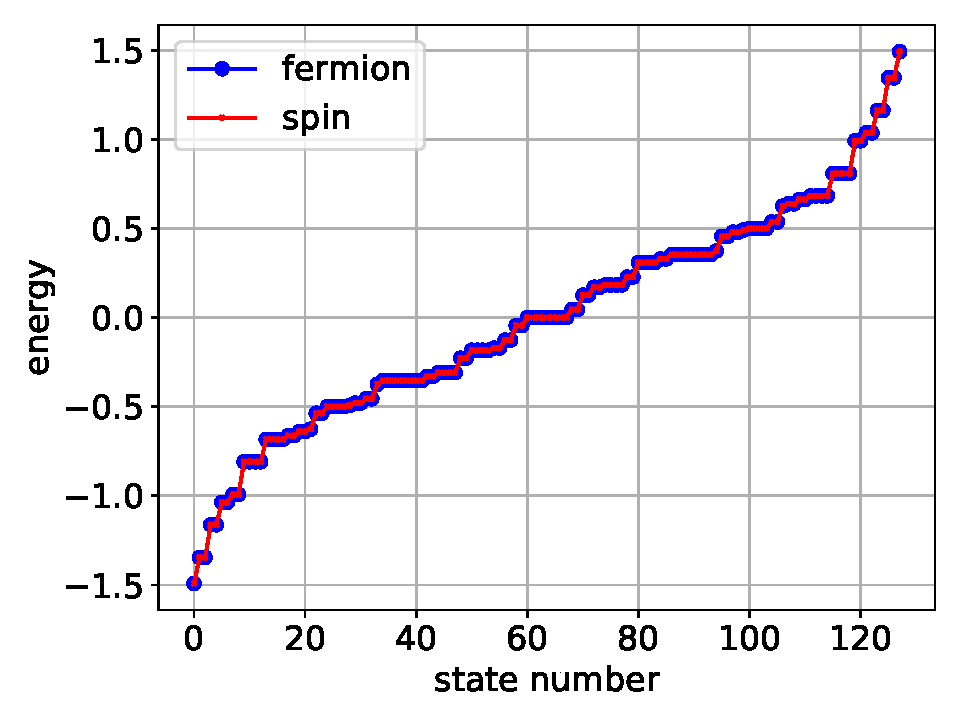
\includegraphics[width=\textwidth]{JW_PBC.pdf}
		\caption{negative spin inversion/PBC sector}
	\end{subfigure}
	\begin{subfigure}[b]{0.496\textwidth}
		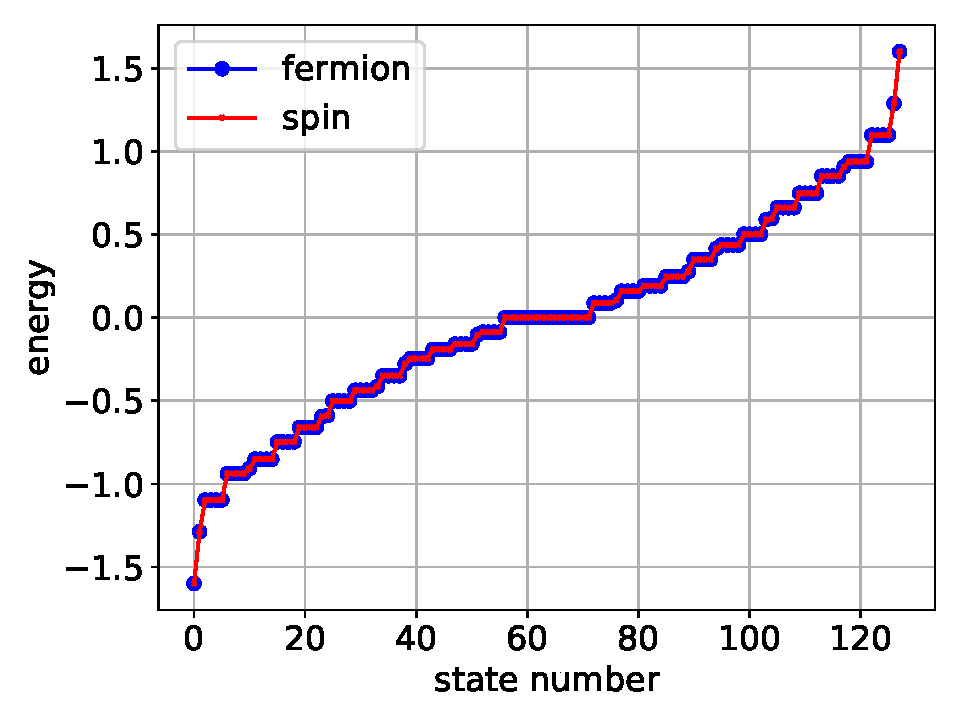
\includegraphics[width=\textwidth]{JW_APBC.pdf}
		\caption{positive spin inversion/APBC sector}
	\end{subfigure}
	\caption{\label{fig:JW} Comparison of the spectra of the spin and fermion representation of the transverse field Ising Hamiltonian in the spin~\eqref{eq:TFIM} and fermion~\eqref{eq:TFIM_fermion} representations. The degeneracy is the spectrum is due to the remaining parity and momentum conservations which are not taken into account (see text). The parameters are $J=1.0$, $h=\sqrt{2}$, and $L=8$.}  
\end{figure} 

\noindent\emph{Code Analysis---}...
\lstinputlisting[firstline=1, lastline=55]{example6.py}

The complete code including the lines that produce Fig.~\ref{fig:example3} is available in Example Code~\ref{code:ex3}.



\subsection{Integrability Breaking in Higher spin transverse field ising model}

This example shows how to:
\begin{itemize}
	\item construct Hamiltonians for Higher spin operators.
	\item find ground state of a Hamiltonian
	\item use obs\_vs\_time function with costume user defined generator to calculate the expectation value of operators as a function of time.
	\item use the new functionality of the basis class to calculate the entanglement entropy for higher spin.
\end{itemize}

\emph{Physics Setup} In the previous section we introduced the TFIM and showed how one can solve the problem using the Jordan-Wigner transformation. This transformation allows one to solve the Hamiltonian exactly. The fact that this solution exists in deeply connected to the notion of Integrability which has implications of how the system responds to a periodic modulation [CITE]. For non-integrable system when periodic driving, energy is no longer conserved and so generically one would expect that the system will heat up to infinite temperature, while in an integrable system, even though energy is not conserved, there is still an extensive number of other conserved quantities which may be conserved under the drive. If this is the case, then the system will not heat up at long times. 

defining two Hamiltonians:
\begin{gather}
	H_{zz} = -J_{zz}\sum_{i=0}^{L-1} S^z_iS^z_{i+1}\\
	H_{x} = -h_x\sum_{i=0}^{L-1}S^x_i
\end{gather}
For both $S_i=1$ and $S_i=1/2$ operators, We will evolve the ground state of $H_{zz}$ with the following piecewise hamiltonian:

\begin{equation}
	H(t)=
	\begin{cases}
		
	\end{cases}
\end{equation}

\subsection{Repulsively Bound Bosons on Translationally Invariant Ladder}

This example shows how to:
\begin{itemize}
	\item construct Hamiltonians for bosonic systems
	\item construct ladder Hamiltonians
	\item using block\_tools module to evolve over several symmetry sectors at once using the block\_ops class
\end{itemize}


\subsection{Fermionic Many-body Localization}

This example shows how to:
\begin{itemize}
	\item construct Hamiltonians for spinful fermions using the tensor\_basis class.
	\item how to use ops\_dict class to construct Hamiltonians with varying parameters.
	\item use new basis functionality to construct simple product states
\end{itemize}


\subsection{Free Particle Systems: the SSH Model}
\label{subsec:free_particle}

This example shows how to
\begin{itemize}
	\item construct free-particle Hamiltonians in real space,
	\item implement translation invariance with a two-site unit cell and construct the single-particle Hamiltonian in momentum space in block-diagonal form,
	\item compute non-equal time correlation functions,
	\item ...
\end{itemize}

\noindent\emph{Physics Setup---}The Su-Schrieffer-Heeger (SSH) model of a free-particle on a dimerised chain is widely used to introduce the concept of edge states, topology, Berry phase, etc., in one spatial dimension. The Hamiltonian is given by
\begin{eqnarray}
H = \sum_{j=0}^{L-1} -(J+(-1)^j\delta J)\left(c_jc^\dagger_{j+1} - c^\dagger_{j}c_{j+1}\right) + \Delta(-1)^jn_j, 
\label{eq:SSH}
\end{eqnarray}
where $\{c_i,c^\dagger_j\}=\delta _{ij}$ obey fermionic commutation relations. The uniform part of the hopping matrix element is $J$, $\delta J$ defines the bond dimerisation, and $\Delta$ is the staggered potential. We assume periodic boundary conditions.

Below, we show how one can use QuSpin to study the physics of free fermions in the SSH chain. One way of doing this would be to work in the many-body (Fock space) basis, see Sec.~???. However, whenever the particles are non-interacting, the exponential scaling of the Hilbert space dimension with the number of lattice sites imposes an artificial limitation on the system sizes one can do. Luckily, with no interactions present, the many-body wave functions factorise in a product of single-particle states. Hence, it is possible to study the behaviour of many free bosons and fermions by simulating the physics of a single particle.

Making use of translation invariance, a straightforward Fourier transformation to momentum space, $a_k = \sqrt{2/L}\sum_{j\ \mathrm{even}}^{L-1} \mathrm e^{-i k j}c_{j}$ and $b_k = \sqrt{2/L}\sum_{j\ \mathrm{odd}}^{L-1}\mathrm e^{-i k j} c_{j}$, casts the SSH Hamiltonian in the following form
\begin{equation}
H \!=\! \sum_{k\in\mathrm{BZ'}} (a^\dagger_k,b^\dagger_k)^t
\left(\begin{array}{cc}
\Delta & -(J+\delta J)\mathrm e^{-i k} - (J-\delta J)\mathrm e^{+i k} \\
-(J+\delta J)\mathrm e^{+i k} - (J-\delta J)\mathrm e^{-i k} & -\Delta
\end{array}
\right)
\left(\! \begin{array}{c}
a_k\\
b_k
\end{array}
\!\right),
\end{equation}
where the reduced Brillouin zone is defined as $\mathrm{BZ'}=[-\pi/2,\pi/2)$. We thus see that the Hamiltonian reduces further to a set of independent $2\times 2$ matrices. The spectrum of the SSH model is gapped, see Fig.~???.

Since we are dealing with free fermions, the ground state is the Fermi sea, $|\mathrm{FS}\rangle$, defined by filling up the lowest band completely. We are interested in measuring the real-space non-equal time correlation function
\begin{equation}
C_{ij}(t) = \langle \mathrm{FS}|n_i(t)n_j(0)|\mathrm{FS}\rangle = \langle \mathrm{FS}(t)|n_i(0)\underbrace{U(t,0)n_j(0)|\mathrm{FS}\rangle}_{|\mathrm{nFS}(t)\rangle}.
\end{equation}
For simplicity, let us focus on a single unit cell. Figure~??? shows the time evolution of $C_{AA}(t)$ and $C_{AB}(t)$. 

\noindent\emph{Code Analysis---}...
\lstinputlisting[firstline=1, lastline=55]{example6.py}

The complete code including the lines that produce Fig.~\ref{fig:example3} is available in Example Code~\ref{code:ex3}.


\subsection{The Gross-Pitaevskii Equation and Nonlinear Time Evolution}
\label{subsec:gen_evolve}

This example shows how to
\begin{itemize}
	\item simulate time-dependent nonlinear equations of motion
	\item use imaginary time dynamics to find a lowest energy configuration
	\item ...
\end{itemize}

\noindent\emph{Physics Setup---}The Gross-Pitaevskii wave equation (GPE) has been shown to govern the physics of weakly-interacting bosonic systems. It constitutes the starting point for studying Bose-Einstein condensates, but can also appear in non-linear optics, and represents the natural description of Hamiltonian mechanics in the wave picture. One of its characteristic features is that it exhibits chaotic classical dynamics, a physical manifestation of the presence of a cubic non-linear term.

Here, we study the time-dependent GPE on a one-dimensional lattice:
\begin{eqnarray}
i\partial_t\psi_j(t) = -J\left( \psi_{j-1}(t) + \psi_{j+1}(t)\right) + \frac{1}{2} \omega_\mathrm{trap}(t)(j-j_0)^2\psi_j(t) + U|\psi_j(t)|^2\psi_j(t),
\label{eq:GPE}
\end{eqnarray}
where $J$ is the hopping matrix element, $\omega_\mathrm{trap}(t)=(\omega_f-\omega_i)t/t_\mathrm{ramp} + \omega_i$ -- the slowly-varying time-dependent harmonic trap frequency over a time scale $t_\mathrm{ramp}$, and $U$ -- the interaction strength. The lattice sites are labelled by $j=0,\dots,L-1$, and $j_0$ is the centre of the 1d chain. We set the lattice constant to unity, and use open boundary conditions.

Whenever $U=0$, the system is non-interacting and the GPE reduces to the Heisenberg EOM for the bosonic field operator $\hat\psi_j(t)$. Thus, for the purposes of using QuSpin to simulate the GPE, it is instructive to cast Eq.~\eqref{eq:GPE} in the following generic form
\begin{equation}
i\partial_t\vec{\psi}(t) = H_\mathrm{sp}(t)\vec{\psi}(t) + U \vec{\psi}^*(t)\circ \vec{\psi}(t)\circ \vec{\psi}(t), 
\end{equation}  
where $[\vec{\psi}(t)]_j = \psi_j(t)$, and $\circ$ represents the element-wise multiplication 
\begin{equation*}
\vec{\psi}(t)\circ \vec{\phi}(t) = \bigg(\psi_0(t)\phi_0(t), \psi_1(t)\phi_1(t),\dots, \psi_{L-1}(t)\phi_{L-1}(t) \bigg)^t.
\end{equation*}
The time-dependent single-particle Hamiltonian in real space is represented as an $L\times L$ matrix, $H_\mathrm{sp}(t)$, which comprises the hopping term, and the harmonic trap.

We want to initiate the time-evolution of the system at $t=0$ in its lowest energy state. To this end, we can define a `ground state' for the GPE equation, in terms of the configuration which minimises the energy of the system:
\begin{eqnarray}
\vec\psi_\mathrm{GS} &=& \inf_{\vec{\psi}} \bigg( \vec{\psi}^t H_\mathrm{sp}(0)\vec{\psi} + \frac{U}{2}\sum_{j=0}^{L-1}|\psi_j|^4\bigg),\nonumber\\
&=&\inf_{\psi_j} \bigg(\sum_{j=0}^{L-1} -J(\psi_{j+1}^*\psi_j + \mathrm{c.c.}) + \frac{1}{2}\omega_\mathrm{trap}(0)|\psi_j|^2 + \frac{U}{2}|\psi_j|^4\bigg).
\end{eqnarray} 
One way to find the configuration $\vec\psi_\mathrm{GS}$, is to solve the GPE in imaginary time ($it\to \tau$), which induces exponential decay in all modes of the system, except for the lowest-energy state. In doing so, we keep the norm of the solution fixed:
\begin{eqnarray}
\partial_{\tau}\vec\varphi(\tau) &=& -\bigg[H_\mathrm{sp}(0)\vec\varphi(\tau) + U \vec\varphi^*(\tau)\circ \vec\varphi(\tau)\circ \vec\varphi(\tau)\bigg],\qquad ||\vec\varphi(\tau)||=\mathrm{const.},\nonumber\\
\vec{\psi}_\mathrm{GS} &=& \lim_{\tau\to\infty}\vec\varphi(\tau)
\end{eqnarray}
Once we have the initial state $\vec\psi_\mathrm{GS}$, we evolve it according to the time-dependent GPE, Eq.~\eqref{eq:GPE}, and track down the time evolution of the condensate density $\rho_j(t)=|\psi_j(t)|^2$. Fig.~??? shows the result.

\noindent\emph{Code Analysis---}...
\lstinputlisting[firstline=1, lastline=55]{example6.py}

The complete code including the lines that produce Fig.~\ref{fig:example3} is available in Example Code~\ref{code:ex3}.

>>>>>>> a944abf73c38bc2c917c9bf9fafc275c144df96a
\section{New Horizons for QuSpin}
\label{sec:outro}

\begin{itemize}
	\item 2D lattices
	\item single-particle Hamiltonian class
	\item Liouville dynamics
\end{itemize}
 

We would much appreciate it if the users could report bugs using the \href{https://github.com/weinbe58/qspin/issues}{issues} forum in the QuSpin online repository.


\section*{Acknowledgements}
We would like to thank L.~Pollet, M.~Kolodrubetz, S.~Capponi ... for various stimulating discussions and for providing comments on the draft. The authors are pleased to acknowledge that the computational work reported on in this paper was performed on the Shared Computing Cluster which is administered by \href{http://www.bu.edu/tech/support/research/}{Boston University's Research Computing Services}. The authors also acknowledge the Research Computing Services group for providing consulting support which has contributed to the results reported within this paper. We would also like to thank \href{https://github.com/}{Github} for providing the online resources to help develop and maintain this project. 

% TODO: include funding information
\paragraph{Funding information}
This work was supported by ???
\begin{appendix}
	
	\section{Installation Guide in a Few Steps}
	\label{app:install}
	
	QuSpin is currently only being supported for Python 2.7 and Python 3.5 and so one must make sure to install this version of Python. We recommend the use of the free package manager \href{https://www.continuum.io/downloads}{Anaconda} which installs Python and manages its packages. For a lighter installation, one can use \href{http://conda.pydata.org/miniconda.html}{miniconda}.
	
	\subsection{Mac OS X/Linux}
	To install Anaconda/miniconda all one has to do is execute the installation script with administrative privilege. To do this, open up the terminal and go to the folder containing the downloaded installation file and execute the following command: 
	\begin{lstlisting}[numbers=none,keywordstyle=\ttfamily]
	$ sudo bash <installation_file>
	\end{lstlisting}
	You will be prompted to enter your password. Follow the prompts of the installation. We recommend that you allow the installer to prepend the installation directory to your PATH variable which will make sure this installation of Python will be called when executing a Python script in the terminal. If this is not done then you will have to do this manually in your bash profile file:
	\begin{lstlisting}[numbers=none,keywordstyle=\ttfamily]
	$ export PATH="path_to/anaconda/bin:$PATH"
	\end{lstlisting}
	
	\underline{\bf Installing via Anaconda.}---Once you have Anaconda/miniconda installed, all you have to do to install QuSpin is to execute the following command into the terminal: 
	\begin{lstlisting}[numbers=none,keywordstyle=\ttfamily]
	$ conda install -c weinbe58 quspin
	\end{lstlisting}
	If asked to install new packages just say `yes'. To keep the code up-to-date, just run this command regularly. 
	
	\underline{\bf Installing Manually.}---Installing the package manually is not recommended unless the above method failed. Note that you must have the Python packages NumPy, SciPy, and Joblib installed before installing QuSpin. Once all the prerequisite packages are installed, one can download the source code from \href{https://github.com/weinbe58/qspin/tree/master}{github} and then extract the code to whichever directory one desires. Open the terminal and go to the top level directory of the source code and execute:
	\begin{lstlisting}[numbers=none,keywordstyle=\ttfamily]  
	$ python setup.py install --record install_file.txt
	\end{lstlisting}
	This will compile the source code and copy it to the installation directory of Python recording the installation location to \texttt{install\_file.txt}. To update the code, you must first completely remove the current version installed and then install the new code. The \texttt{install\_file.txt} can be used to remove the package by running:  
	\begin{lstlisting}[numbers=none,keywordstyle=\ttfamily]  
	$ cat install_file.txt | xargs rm -rf. 
	\end{lstlisting}
	
	\subsection{Windows}
	To install Anaconda/miniconda on Windows, download the installer and execute it to install the program. Once Anaconda/miniconda is installed open the conda terminal and do one of the following to install the package:
	
	\underline{\bf Installing via Anaconda.}---Once you have Anaconda/miniconda installed all you have to do to install QuSpin is to execute the following command into the terminal: 
	\begin{lstlisting}[numbers=none,keywordstyle=\ttfamily]
	> conda install -c weinbe58 quspin
	\end{lstlisting}
	If asked to install new packages just say `yes'. To update the code just run this command regularly. 
	
	\underline{\bf Installing Manually.}---Installing the package manually is not recommended unless the above method failed. Note that you must have NumPy, SciPy, and Joblib installed before installing QuSpin. Once all the prerequisite packages are installed, one can download the source code from \href{https://github.com/weinbe58/qspin/tree/master}{github} and then extract the code to whichever directory one desires. Open the terminal and go to the top level directory of the source code and then execute:  
	\begin{lstlisting}[numbers=none,keywordstyle=\ttfamily]
	> python setup.py install --record install_file.txt
	\end{lstlisting}
	This will compile the source code and copy it to the installation directory of Python and record the installation location to \texttt{install\_file.txt}. To update the code you must first completely remove the current version installed and then install the new code. 
	
	
	\section{Basic Use of Command Line to Run Python}
	\label{app:cmd_line}
	
	In this appendix we will review how to use the command line for Windows and OS X/Linux to navigate your computer's folders/directories and run the Python scripts.
	
	\subsection{Mac OS X/Linux}
	Some basic commands:
	
	\begin{itemize}
		\item change directory:
		\begin{lstlisting}[numbers=none,keywordstyle=\ttfamily]
		$ cd < path_to_directory >
		\end{lstlisting}
		\item list files in current directory:
		\begin{lstlisting}[numbers=none,keywordstyle=\ttfamily]
		$ ls 
		\end{lstlisting}
		list files in another directory:
		\begin{lstlisting}[numbers=none,keywordstyle=\ttfamily]
		$ ls < path_to_directory >
		\end{lstlisting}
		\item make new directory:
		\begin{lstlisting}[numbers=none,keywordstyle=\ttfamily]
		$ mkdir <path>/< directory_name >
		\end{lstlisting}
		\item copy file:
		\begin{lstlisting}[numbers=none,keywordstyle=\ttfamily]
		$ cp < path >/< file_name > < new_path >/< new_file_name >
		\end{lstlisting}
		\item move file or change file name:
		\begin{lstlisting}[numbers=none]
		$ mv < path >/< file_name > < new_path >/< new_file_name >
		\end{lstlisting}
		\item remove file:
		\begin{lstlisting}[numbers=none,keywordstyle=\ttfamily]
		$ rm < path_to_file >/< file_name >
		\end{lstlisting}
		
	\end{itemize}
	Unix also has an auto complete feature if one hits the TAB key. It will complete a word or stop when it matches more than one file/folder name. The current directory is denoted by "." and the directory above is "..".
	%
	Now, to execute a Python script all one has to do is open your terminal and navigate to the directory which contains the python script. To execute the script just use the following command:
	\begin{lstlisting}[numbers=none,keywordstyle=\ttfamily]
	$ python script.py
	\end{lstlisting}
	It's that simple!
	
	\subsection{Windows}
	Some basic commands:
	
	\begin{itemize}
		\item change directory:
		\begin{lstlisting}[numbers=none,keywordstyle=\ttfamily]
		> cd < path_to_directory >
		\end{lstlisting}
		\item list files in current directory:
		\begin{lstlisting}[numbers=none,keywordstyle=\ttfamily]
		> dir
		\end{lstlisting}
		list files in another directory:
		\begin{lstlisting}[numbers=none,keywordstyle=\ttfamily]
		> dir < path_to_directory >
		\end{lstlisting}
		\item make new directory:
		\begin{lstlisting}[numbers=none,keywordstyle=\ttfamily]
		> mkdir <path>\< directory_name >
		\end{lstlisting}
		\item copy file:
		\begin{lstlisting}[numbers=none,keywordstyle=\ttfamily]
		> copy < path >\< file_name > < new_path >\< new_file_name >
		\end{lstlisting}
		\item move file or change file name:
		\begin{lstlisting}[numbers=none,keywordstyle=\ttfamily]
		> move < path >\< file_name > < new_path >\< new_file_name >
		\end{lstlisting}
		\item remove file:
		\begin{lstlisting}[numbers=none,keywordstyle=\ttfamily]
		> erase < path >\< file_name >
		\end{lstlisting}
		
	\end{itemize}
	Windows also has a auto complete feature using the TAB key but instead of stopping when there multiple files/folders with the same name, it will complete it with the first file alphabetically. The current directory is denoted by "." and the directory above is "..".
	
	\subsection{Execute Python Script (any operating system)}
	%
	To execute a Python script all one has to do is open up a terminal and navigate to the directory which contains the Python script. Python can be recognised by the extension \texttt{.py}. To execute the script just use the following command:
	\begin{lstlisting}[numbers=none,keywordstyle=\ttfamily]
	python script.py
	\end{lstlisting}
	It's that simple!
	
	\newpage
	
	\section{Package Documentation}
	\label{app:doc}
	In QuSpin quantum many-body operators are represented as matrices. The computation of these matrices are done through custom code written in Cython. Cython is an optimizing static compiler which takes code written in a syntax similar to Python, and compiles it into a highly efficient C/C\texttt{++} shared library. These libraries are then easily interfaced with Python, but can run orders of magnitude faster than pure Python code~\cite{Cython}. The matrices are stored in a sparse matrix format using the sparse matrix library of SciPy~\cite{SciPy_package}. This allows QuSpin to easily interface with mature Python packages, such as NumPy, SciPy, any many others. These packages provide reliable state-of-the-art tools for scientific computation as well as support from the Python community to regularly improve and update them~\cite{NumPy,Python_computing_1,Python_computing_2,SciPy_package}. Moreover, we have included specific functionality in QuSpin which uses NumPy and SciPy to do many desired calculations common to ED studies, while making sure the user only has to call a few NumPy or SciPy functions directly. The complete up-to-date documentation for the package is available online under:\\
	
	\href{https://github.com/weinbe58/QuSpin/#quspin}{https://github.com/weinbe58/QuSpin/\#quspin}\\
	
	\newpage
	\section{Complete Example Codes}
	\label{app:scripts}
	
	In this appendix, we give the complete python scripts for the dix examples discussed in Sec.~\ref{sec:examples}. In case the reader has trouble with the TAB spaces when copying from the code environments below, the scripts can be downloaded from github at: \center{ \href{https://github.com/weinbe58/QuSpin/tree/master/examples}{https://github.com/weinbe58/QuSpin/tree/master/examples}}
	
	
	%\lstinputlisting[label=code:ex0,caption=Exact Diagonalisation of the XXZ Model]{example0.py}
	%\newpage
	%\lstinputlisting[label=code:ex1,caption=Adiabatic Control of Parameters in MBL Phases]{example1.py}
	%\newpage
	%\lstinputlisting[label=code:ex2,caption=Heating in Periodically Driven Spin Chains]{example2.py}
	%\newpage
	%\lstinputlisting[label=code:ex3,caption=Quantised Light-Atom Interactions in the Semi-classical Limit]{example3.py}
	
	
\end{appendix}


% TODO: 
% Provide your bibliography here. You have two options:
%\bibliographystyle{SciPost_bibstyle}
%\bibliographystyle{abbrv}

\begin{comment}
% FIRST OPTION - write your entries here directly, following the example below, including Author(s), Title, Journal Ref. with year in parentheses at the end, followed by the DOI number.
\begin{thebibliography}{99}
\bibitem{1931_Bethe_ZP_71} H. A. Bethe, {\it Zur Theorie der Metalle. i. Eigenwerte und Eigenfunktionen der linearen Atomkette}, Zeit. f{\"u}r Phys. {\bf 71}, 205 (1931), \doi{10.1007\%2FBF01341708}.
\bibitem{arXiv:1108.2700} P. Ginsparg, {\it It was twenty years ago today... }, \url{http://arxiv.org/abs/1108.2700}.
\end{thebibliography}
\end{comment}

% SECOND OPTION:
% Use your bibtex library
%\bibliographystyle{SciPost_bibstyle.bst} % Include this style file here only if you are not using our template
\bibliography{qspin}

\nolinenumbers

\end{document}
